\section{Practical}
  This paper demonstrated hosting a web application using a sample web site provided by AWS. The website consists of a number of web pages which allow the user to register, verify their email address and sign in. The logic for these functions is provided by the static web pages and AWS Cognito. Once, registered and logged in, the user is directed to a global map at which point the user can enter their location in order to request a unicorn. The request logic is handled by AWS lambda. This function will return the response from the request to the client while also recording the details of the request in a backend database, implemented using DynamoDB. 
  

  \subsection{Static Web Content on S3}
  S3 hosts the static portion of the web application. This not only includes static \textit{html} pages but also client side JavaScript, for example the user authentication logic which runs on the client. Therefore,the first step was to create an S3 bucket. This was achieved with the following command:
  
  \noindent\begin{minipage}{\textwidth}
    \begin{lstlisting}[caption={Create Bucket},label=create-bucket,language=bash]
    aws s3api create-bucket --bucket cloud-infra-wild-rydes --region eu-west-1 --region eu-west-1 --create-bucket-configuration LocationConstraint=eu-west-1
    \end{lstlisting}
  \end{minipage}
  
  \noindent Once the bucket was created the static content was added. As mentioned above, the static website is provided by AWS. This means the content can easily copied to the bucket from the provided AWS source bucket:
  
  \noindent\begin{minipage}{\textwidth}
    \begin{lstlisting}[caption={Adding Static Content to S3 Bucket},label=populate-bucket,language=bash]
    aws s3 sync s3://wildrydes-us-east-1/WebApplication/1_StaticWebHosting/website s3://cloud-infra-wild-rydes --region eu-west-1
    \end{lstlisting}
  \end{minipage}
  
   
  \subsubsection{Allow Public Access}
  
    \noindent In order to make the website visible to a browser the bucket needs to be configured to hosts static web content. First the bucket needs to be given public read permissions. This is done by creating a bucket policy which grants anonymous read access to all assets in the bucket:
    
    \noindent\begin{minipage}{\textwidth}
      \begin{lstlisting}[caption={Add Bucket Read Policy},label=bucket-read,language=bash]
      aws s3api put-bucket-policy --bucket cloud-infra-wild-rydes --policy file://bucket-policy.json

      bucket-policy.json >
      {
        "Version": "2012-10-17",
        "Statement": [
          {
            "Effect": "Allow",
            "Principal": "*",
            "Action": "s3:GetObject",
            "Resource": "arn:aws:s3:::cloud-infra-wild-rydes/*"
          }
        ]
      }      
      \end{lstlisting}
    \end{minipage}
    
    \noindent Finally, the bucket was configured for static website hosting:
    
    \noindent\begin{minipage}{\textwidth}
      \begin{lstlisting}[caption={Configure Bucket for Static Website Hosting},label=bucket-hosting,language=bash]
      aws s3 website s3://cloud-infra-wild-rydes/ --index-document index.html
      \end{lstlisting}
    \end{minipage}
    
    \noindent The bucket configuration as now complete and the web site can be view by visiting the buckets URL.
    
    \begin{figure}[H]
      \caption{S3 Bucket Static Web Hosting}
      \centering
      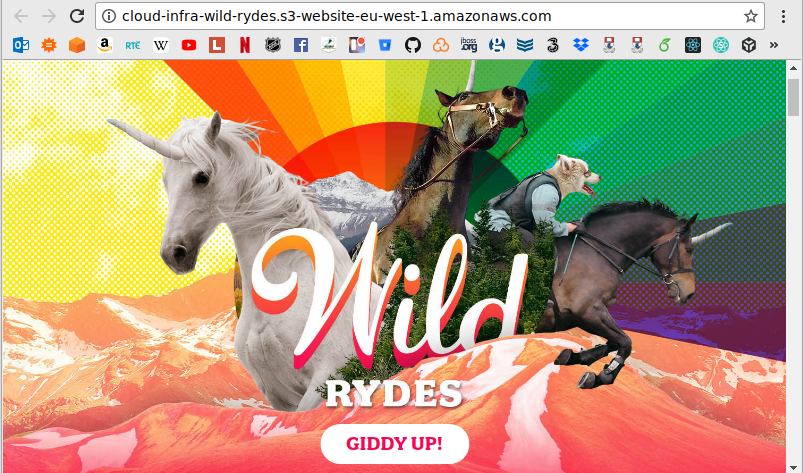
\includegraphics[width=0.8\textwidth,keepaspectratio]{static-web-hosting}
      \label{fig:static-web-hosting}
    \end{figure}
    
    \noindent However, once Cognito is configured, the IDs of some of their resources needs to be added to the bucket in order client side JavaScript to communicate with them. These IDs must be added to the \textit{config.js} file within the bucket to allow the client-side scripting to authentication and verify against the user pool. Therefore, this file was download so that it could be completed later. 
    
    \noindent\begin{minipage}{\textwidth}
      \begin{lstlisting}[caption={Download config.js},label=download-config,language=bash]
      aws s3 cp s3://cloud-infra-wild-rydes/js/config.js config.js
      \end{lstlisting}
    \end{minipage}
  
  \subsection{User Management with Cognito}
  
    \subsubsection{User Pool}
    For this exercise user authentication with Cognito will be provided by a user pool. This is a database of users maintained by Cognito. When a user registers they are added they are sent a verification email including a code. They must then visit the verification page and enter the code at which point the are add to the user pool and can now sign into the app.
    
    A user pool was created using the following command:
    
    \noindent\begin{minipage}{\textwidth}
      \begin{lstlisting}[caption={Create User Pool},label=create-user-pool,language=bash]
      aws cognito-idp create-user-pool --pool-name wild-rydes-user-pool --auto-verified-attributes email --policies file://password-policy.json --schema '{"Name":"email","Required":true,"AttributeDataType":"String"}'
    
      password-policy.json >
        {
        "PasswordPolicy": {
          "MinimumLength": 8,
          "RequireUppercase": true,
          "RequireLowercase": true,
          "RequireNumbers": true,
          "RequireSymbols": false
        }
      }
  
      \end{lstlisting}
    \end{minipage}
    This command creates a user pool with a number of configurations:
    \begin{itemize}
      \item Verification is implemented via email (SMS is also an option)
      \item A password policy is enforced
      \item The email attribute is required
    \end{itemize}
    
  \subsubsection{App Client}
    
    Next an app client (or user pool client) is created. The app client allows the the web application to call unauthenticated API's or functions in Cognito such as \textit{Register} and \textit{Sign in} \citep{awsAppClient}. The app client was configured as follows, including the Pool Id of the pool created above:
    
    \noindent\begin{minipage}{\textwidth}
      \begin{lstlisting}[caption={Create App Client},label=app-client,language=bash]
      aws cognito-idp create-user-pool-client --user-pool-id eu-west-1_yXmbzV1SM --client-name wild-rydes-web-app --no-generate-secret
      \end{lstlisting}
    \end{minipage}
    
    \noindent 
    Finally, the Pool ID and the App Client ID are added to the \textit{config.js} file for the web applications static files.
    

  \subsection{DynamoDB Setup}
  The details of all rides requested are saved in the backend database. This consisted of a DynamoDB table. The table was set up using the follwing command:

  \noindent\begin{minipage}{\textwidth}
    \begin{lstlisting}[caption={Create DynamoDB Table},label=create-table,language=bash]
    aws dynamodb create-table --table-name Rides --attribute-definitions AttributeName=RideId,AttributeType=S --key-schema AttributeName=RideId,KeyType=HASH --provisioned-throughput ReadCapacityUnits=5,WriteCapacityUnits=5
    \end{lstlisting}
  \end{minipage}
  
  \noindent This command creates the table \textit{Rides} with the Primary Key \textit{RideId} which is of type string.
  
  \subsection{IAM Role}
  In order for an AWS Lambda function to run it needs to correct permissions to execute and interface with any necessary AWS services. In this the case the function needs to be able to make entries into a DynamoDB table. The function does this by assuming a Role \citep{awsLambdaPermission}. Accordingly, an IAM role was created with the following policies attached:
  \begin{itemize}
    \item AWS Lambda Basic Execution Role
    \item DynamoSB Write Access
  \end{itemize}
  This was created on the AWS console.
  
  \subsection{Lambda Function}
    The next step was to create the serverless backend for the web app. This simple app consists of only a single backend function, i.e. request a unicorn. This is provided by AWS Lambda. The function was configured with the following attributes:
    \begin{itemize}
      \item \textbf{Runtime: } The runtime environment which should be used to run the function. This function should be run in NodeJS. However, other options such as Python and Java are available allowing functions to be written in a variety of languages.
      \item \textbf{Role: } The role which the function will assume in order to execute with the correct permissions. It is configured with the ARN of the role created above.
      \item \textbf{Handler: } The entrypoint for the function. i.e. the exact function within the provided file(s) which whould run then the Lambda function is called.
      \item \textbf{Code: } The code of the Lambda function. When the function is created using the CLI, the code can provided as a zipped file in S3 which Lambda will retrieve and unzip.
    \end{itemize}
    
    \noindent\begin{minipage}{\textwidth}
      \begin{lstlisting}[caption={Lambda Function},label=create-lambda-function,language=bash]
      aws lambda create-function --function-name RequestAUnicorn --runtime nodejs6.10 --role arn:aws:iam::806626264653:role/WildRydesLambda --handler index.handler --code S3Bucket=cloud-infra-lambda-function,S3Key=index.js.zip
      \end{lstlisting}
    \end{minipage}

  \subsection{API Gateway}
  Due to the complex nature or creating and configuring the API, these steps were carried out via the AWS console. Configuring a the API consisted of a number of steps.
  
  \subsubsection{REST API}
  The first step was to create a rest API. This is shown in \autoref{fig:rest}.
  
  \begin{figure}[H]
    \caption{Creating the REST API}
    \centering
    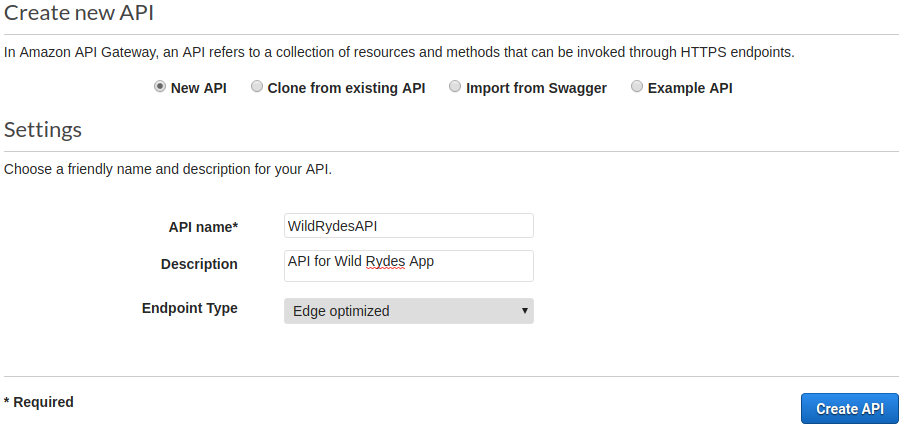
\includegraphics[width=0.8\textwidth,keepaspectratio]{create-api}
    \label{fig:rest}
  \end{figure}
  
  
  \subsubsection{Authorizor for User Pool}
  The API endpoint to be created is for the \textit{RequestAUnicorn}  Lambda function. Users can only access the necessary web page to make this call after authenticating. Therefore, the API Gateway needs a method on ensuring on authenticated request are accepted. This is achieved using an Authorizer connected to the Cognito user pool created above. JSON Web Tokens (JWT) are used to verify authorisation of requests after users have authenticated. The client includes their token with the request to the API and the Authorizer  verified this token with the Cognito user pool. Configuring the Authorizer on AWS requires that the header used for authentication be specified. 
  
  \autoref{fig:authorizer} shows the \textit{Authorization} header is chosen. This is the header which will be used by the API to send user token to the Cognito user pool to verification. Also, shown is the user pool created above 
  
  \begin{figure}[H]
    \caption{Creating the Authorizer}
    \centering
    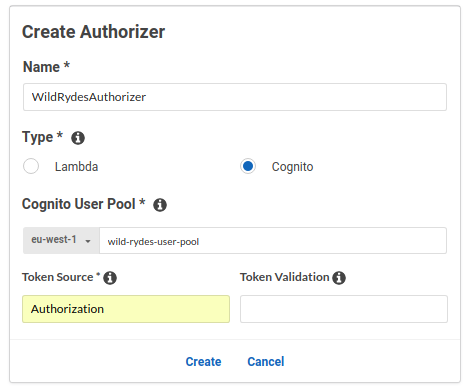
\includegraphics[width=0.65\textwidth,keepaspectratio]{create-authorizer}
    \label{fig:authorizer}
  \end{figure}  

  \subsubsection{POST Resource Method}
  The API was then populated with an endpoint. For this app there is only one endpoint i.e. \textit{/ride}. The endpoints will accept only HTTP Post requests. Endpoints are defined in API Gateway be as resources. They are created relative to the root domain or parent resources for the purposes of mirroring URL paths. In this case the ride resources' parent is the root domain.
   
  When creating the resource is was important to enable CORS. CORS, or Cross Origin Resource Scripting, is a security concept concerned with APIs called by sources in a different domain. Browsers often restrict API calls to other domains for security reasons. Enabling CORS allows a client running access resources in a different domain via the REST API. This is achieved by adding CORS headers to the request and enabling CORS on the target domain \citep{mozilla}. In this case, client side files are being server from S3, where API request are directed to API Gateway. Therefore, CORS must be enable on the REST API.
  
  \begin{figure}[H]
    \caption{Creating the REST API}
    \centering
    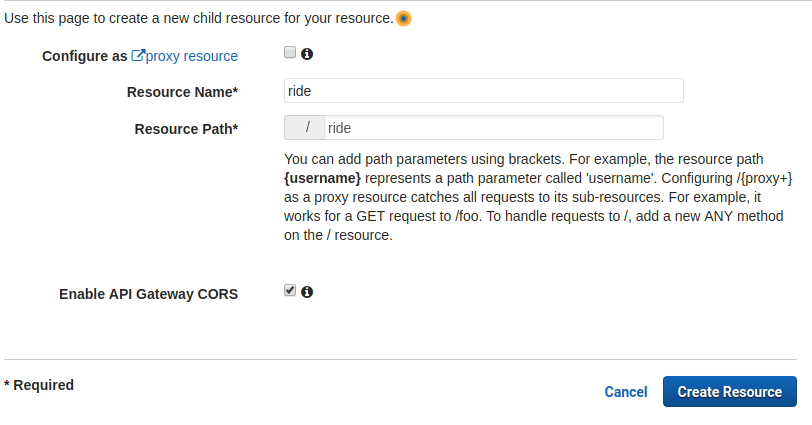
\includegraphics[width=\textwidth,keepaspectratio]{resource}
    \label{fig:resource}
  \end{figure}
  
  With the resource created the HTTP method can be added. The \textit{ride} resource accepts a POST method, as the user sends their location in order to request a unicorn. The lambda function created earlier was selected as the integration for the POST method. Also, the authorizer created above was added to the method to perform the verification against the user pool.
  
  \begin{figure}[H]
    \caption{Creating the POST Method}
    \centering
    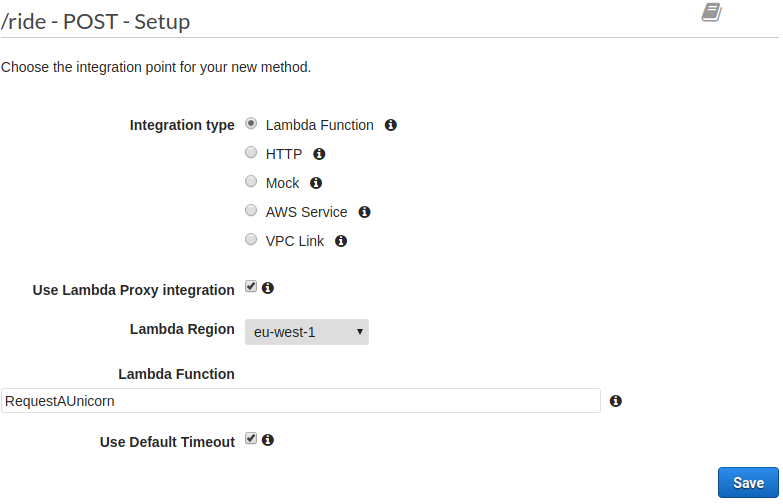
\includegraphics[width=0.75\textwidth,keepaspectratio]{post}
    \label{fig:post}
  \end{figure}
    
  \begin{figure}[H]
    \caption{Authorising the POST Method}
    \centering
    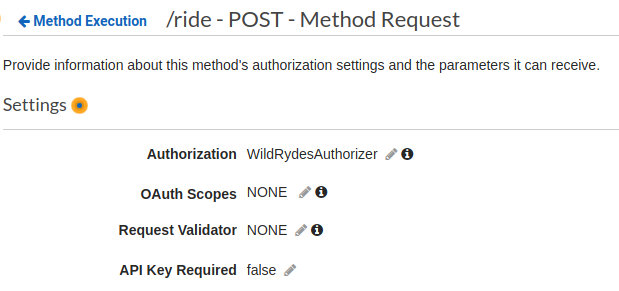
\includegraphics[width=0.75\textwidth,keepaspectratio]{authorise-post}
    \label{fig:authorise-post}
  \end{figure}
  
  \noindent Viewing the Lambda function on the console now indicates that the API Gateway has been added as a trigger for the function.
  
  \begin{figure}[H]
    \caption{Authorising the POST Method}
    \centering
    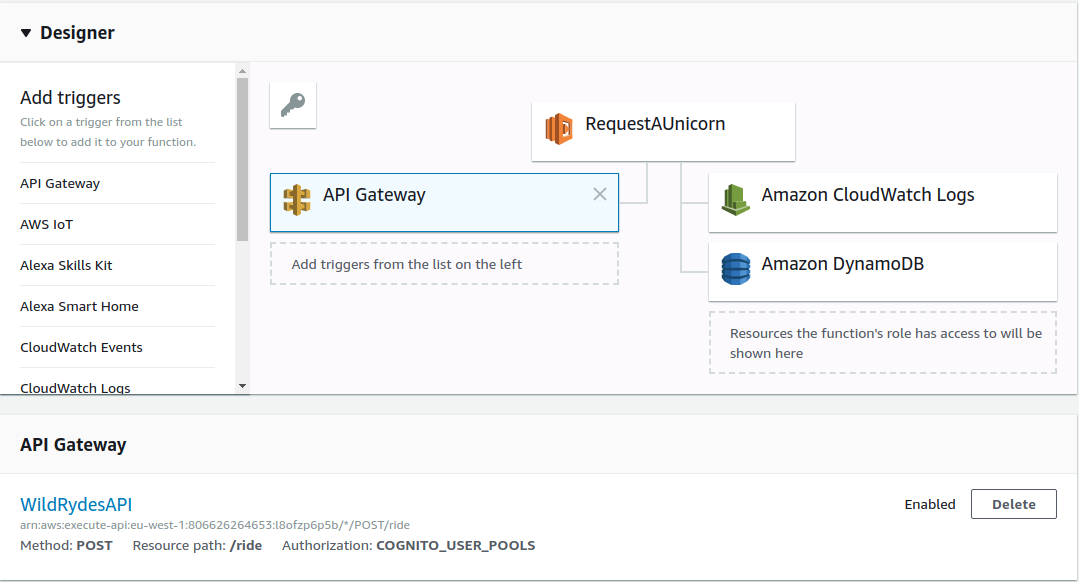
\includegraphics[width=\textwidth,keepaspectratio]{trigger}
    \label{fig:trigger}
  \end{figure}
  
  \subsubsection{Deploy API}
  The final step was to deploy the API. This created a URL at which the API can be targetted. This must be recorded and added to the \textit{config.js} file for the client side scripts in the S3 bucket. This simply consists of clicking \textit{Deploy} and adding a stage name, in this case \textit{prod}.
  
  \begin{figure}[H]
    \caption{Authorising the POST Method}
    \centering
    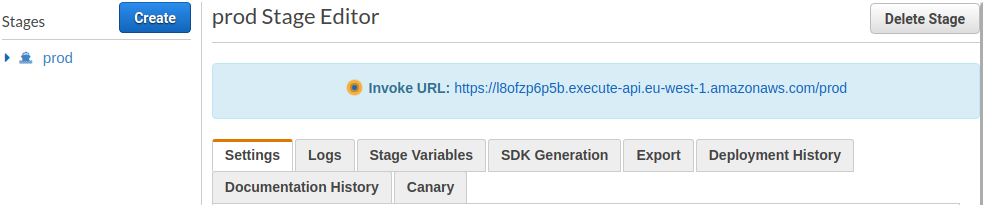
\includegraphics[width=\textwidth,keepaspectratio]{deploy}
    \label{fig:deploy}
  \end{figure}
  
  \subsection{Updating S3}
  With the serverless backend complete the final stage is to update the \textit{config.js} file in the bucket. This final configuration is shown in below:
  
  \noindent\begin{minipage}{\textwidth}
    \begin{lstlisting}[caption={Client Side Scripting config.js},label=confid-js,language=bash]
    window._config = {
      cognito: {
        userPoolId: 'eu-west-1_yXmbzV1SM', // e.g. us-east-2_uXboG5pAb
        userPoolClientId: '62tba8dssa0036ig0r30hklbdm', // e.g. 25ddkmj4v6hfsfvruhpfi7n4hv
        region: 'eu-west-1' // e.g. us-east-2
      },
      api: {
        invokeUrl: 'https://l8ofzp6p5b.execute-api.eu-west-1.amazonaws.com/prod' // e.g. https://rc7nyt4tql.execute-api.us-west-2.amazonaws.com/prod',
      }
    };
    \end{lstlisting}
  \end{minipage}
  
  \noindent The configuration file was copied to the bucket using the following command:
  
  \noindent\begin{minipage}{\textwidth}
    \begin{lstlisting}[caption={Copy config.js to bucket},label=copy-confid-js,language=bash]
    aws s3 cp config.js s3://cloud-infra-term-paper/js/config.js
    \end{lstlisting}
  \end{minipage}
    
